\section{Question 4: Government Budget Change from the Reform}

\subsection*{Method}

To calculate how the government budget changes when switching from joint to individual taxation, we compute the total lifetime tax revenue per household under each system. For each period $t$, the average tax payment across all simulated households is:
%
\begin{equation}
    \text{Rev}_t = \mathbb{E}\left[\text{tax}_{i,t}\right] = \frac{1}{N} \sum_{i=1}^{N} \text{tax}_{i,t}
\end{equation}
%
where $N$ is the number of simulated households. Under joint taxation, $\text{tax}_{i,t} = T_{\text{joint}}(Y_{1,i,t} + Y_{2,i,t})$, and under individual taxation, $\text{tax}_{i,t} = T_{\text{indiv}}(Y_{1,i,t}) + T_{\text{indiv}}(Y_{2,i,t})$.

The total lifetime revenue per household is then the sum over all periods:
%
\begin{equation}
    G = \sum_{t=0}^{T-1} \text{Rev}_t
\end{equation}
%
The budget change from the reform is:
%
\begin{equation}
    \Delta G = G^{\text{indiv}} - G^{\text{joint}}
\end{equation}

\subsection*{Results}

From our simulation we get:

\begin{center}
\begin{tabular}{l r}
\hline
Lifetime revenue, joint taxation      & 3{,}610.3 \\
Lifetime revenue, individual taxation & 5{,}342.3 \\
\hline
Budget change ($\Delta G$)            & $+$1{,}732.1 \\
Change in percent                     & $+$47.98\% \\
\hline
\end{tabular}
\end{center}

So switching to individual taxation actually \emph{increases} government revenue by about 48\%. This happens because the individual tax system encourages member 2 to work more (as discussed in Question~3), which raises total household income and therefore total tax payments, even though the marginal tax rate on the secondary earner is lower.

% ---------------------------------------------------------------
% PLACEHOLDER PLOT
% ---------------------------------------------------------------
% \begin{center}
% \fbox{\parbox{0.85\textwidth}{
% \textbf{[INSERT PLOT: Per-period average tax revenue]}\\[6pt]
% Line plot with two series: average tax revenue per household under joint taxation and under individual taxation, for each period $t = 0, \ldots, 9$.
% X-axis: period $t$. Y-axis: average tax revenue.
% The individual taxation line should be above the joint taxation line in most or all periods.
% }}
% \end{center}

\begin{figure}
    \centering
    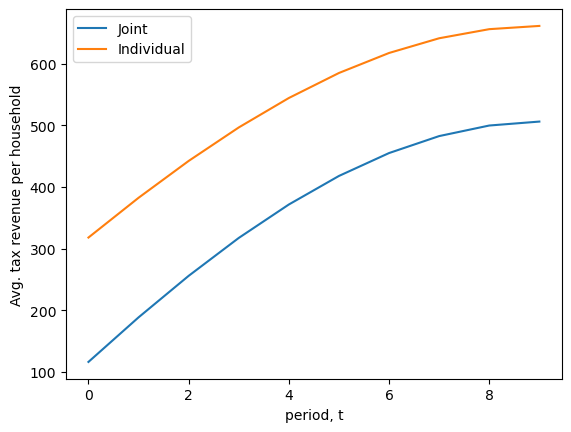
\includegraphics[width=0.5\linewidth]{Billeder/Per-period average tax revenue.png}
    \caption{Caption}
    \label{fig:placeholder}
\end{figure}

\subsection*{Note on Discounting}

If we discount future revenue using the household's discount factor $\beta = 0.98$, the present value of the budget change is 1{,}592.3, which is still a large positive number. This confirms that the revenue gain is not driven by a few late periods but is present throughout the life cycle.
